\section{質疑や議論を通したSIL2LinuxMPコミュニティへのコントリビューション}
本節では、2015年4月からこれまで\acrshort{sil2linuxmp}活動を通してコミュニティへ働きかけた内容を記載する。
\acrshort{sil2linuxmp}プロジェクトにおける主なコミュニケーション手段はメーリングリストと\acrshort{git}である。
プロジェクトに対する活動は各参加者の主体性に任されている状況であり、全ての活動はメーリングリストおよび\acrshort{git}の履歴に残り
最終的に\acrshort{sil2linuxmp}の成果として参照される。
このようなオープンなプロジェクトでは、有益なコントリビューションを多く残している参加者ほどコミュニティに認知される。
\ref{contribution}節で述べたように、近年はオープンなコミュニティで認知されること自体が長期的に価値のある投資としての意味を持つ。
\acrshort{oss}に対する機能安全のノウハウを得るという目的と並んで、日立の\acrshort{sil2linuxmp}への貢献を示すため、
また筆者自身が\acrshort{oss}活動の進め方を理解するため、研修期間を通してメーリングリストと\acrshort{git}での活動を活発に行うことを意識した。
\subsection{メーリングリスト上での活動}
\label{mailinglist}
\href{http://lists.osadl.org/pipermail/sil2linuxmp/}{\acrshort{sil2linuxmp}メーリングリスト} \cite{mail}はコミュニティでの議論や何らかの告知が行われる公な場である。
日立からは、\gls{srs}などの\acrshort{sil2linuxmp}ドキュメントとコンプライアンスルートおよび各種検証手法の不明点の質問をするため、また日立が行った技術調査・検討内容の報告をするめにメーリングリストへの投稿を継続的に行った。
表\ref{mailindividual}は、メーリングリストへの投稿者別に2015年4月$\sim$ 2016年3月までの投稿数が多い順で投稿者メールアドレスをリストした結果である。
日立は4名から投稿があり、そのうち筆者(kotaro.hashimoto.jv@hitachi.com)は36投稿でプロジェクト全参加者中で2番目に投稿数が多かった。
1、3番目に投稿数が多いder.herr@hofr.at (Nicholas Mc Guire)とandreas.platschek@opentech.atは\acrshort{sil2linuxmp}プロジェクトの主催メンバである。
これまでこのメーリングリストでは、日立が発した質問に対してNicholasやAndreasが回答しそれに他の参加者が反応して議論が膨らんでいく、という形式で話が進むケースが多かった。
\begin{table}[H]
  \caption{個人別\acrshort{sil2linuxmp}メーリングリスト投稿数ランキング(2015年4月$\sim$ 2016年3月)}
  \label{mailindividual}
  \centering
  \begin{tabular}{l|l}
    \multicolumn{1}{c|}{投稿数} & \multicolumn{1}{c}{投稿者メールアドレス} \\
    \hline 
    40 & der.herr@hofr.at (Nicholas Mc Guire) \\
    \textbf{36} & \textbf{kotaro.hashimoto.jv@hitachi.com} \\
    16 & andreas.platschek@opentech.at (andi@opentech.at 含む) \\
    15 & Mandar.Pitale@bmw-carit.de \\
    13 & julia.lawall@lip6.fr \\
    \textbf{13} & \textbf{krishnaji@hitachi.co.in} \\
    12 & C.Emde@osadl.org \\
    8 & Lukas.Bulwahn@bmw-carit.de \\
    7 & georg.schiesser@opentech.at (george.schiesser@gmail.com 含む) \\
    6 & Bernhard.Noelte@tuev-sued.de \\
    3 & office@osadl.org \\
    2 & Georg.Waibel@sensor-technik.de \\
    2 & KaziKhaled.Al-Zahid@bmw-carit.de \\
    2 & Tilmann.Ochs@bmw.de \\
    1 & Ursula.Braun@osadl.org \\
    1 & Tilmann.Ochs@bmw-carit.de \\
    \textbf{1} & \textbf{masami.hiramatsu.pt@hitachi.com} \\
    1 & Quirin.Gylstorff@kuka.com \\
    1 & dvhart@linux.intel.com \\
    1 & khoroshilov@ispras.ru \\
    \textbf{1} & \textbf{pradyumna@hitachi.co.in} \\
    1 & Kai-Daniel.Niestroj@sensor-technik.de \\
    1 & Christian.Hartmann@kuka.com \\
    1 & jeremiah.foster@pelagicore.com \\
    1 & Mandar.Pitale@bmw.de
  \end{tabular}
\end{table}
\par
表\ref{mailcompany}は投稿者のメールアドレス情報を元に企業別で投稿数を集計した結果である。
日立は\acrshort{sil2linuxmp}プロジェクト主催元の\acrshort{ot}に続いて51投稿で、プロジェクト全参加企業中で2番目に投稿数が多かった。
\begin{table}[H]
  \caption{企業別\acrshort{sil2linuxmp}メーリングリスト投稿数ランキング(2015年4月$\sim$ 2016年3月)}
  \label{mailcompany}
  \centering
  \begin{tabular}{l|l}
    \multicolumn{1}{c|}{投稿数} & \multicolumn{1}{c}{投稿者メールアドレス} \\
    \hline 
    63 & opentech.at (hofr.at 含む) \\
    \textbf{51} & \textbf{hitachi.com} (hitachi.co.in 含む) \\
    29 & bmw.de (bmw-carit.de 含む) \\
    16 & osadl.org \\
    13 & lip6.fr (\acrshort{inria}) \\
    6 & tuev-sued.de \\
    3 & sensor-technik.de \\
    2 & kuka.com \\
    1 & pelagicore.com \\
    1 & linux.intel.com \\
    1 & ispras.ru
  \end{tabular}
\end{table}
\par
表\ref{thread}はメーリングリストでの話題(スレッド)別に各話題における投稿数を集計した結果である。
これらのうち、日立が初めに投稿した質問または提案で議論が始まったものは右端に\checkmark{}を付けている。
\begin{table}[H]
%  \footnotesize
  \small
  \caption{スレッド別\acrshort{sil2linuxmp}メーリングリスト投稿数ランキング(2015年4月$\sim$ 2016年3月)}
  \label{thread}
  \centering
  \begin{tabular}{l|l|l}
    \multicolumn{1}{c|}{投稿数} & \multicolumn{1}{c|}{スレッドタイトル名(の一部)} & \multicolumn{1}{c}{日立の投稿で議論が始まったもの} \\
    \hline 
    \textbf{19} & \textbf{Question about SRS and verification strategy} & \checkmark{} \\
    16 & Return Oriented Programming (ROP) & \\
    11 & Next SIL2LinuxMP meeting in September & \\
    \textbf{10} & \textbf{How could we qualify a toolchain (T3 off-line} & \checkmark{} \\
    \textbf{10} & \textbf{SRS question: How will COTS upgrade process be} & \checkmark{} \\
    \textbf{10} & \textbf{Pruning function call graph} & \checkmark{} \\
    \textbf{8} & \textbf{Gray box Analysis approach} & \checkmark{} \\
    8 & Preliminary safety concept available? & \\
    \textbf{8} & \textbf{Results of Static analysis on Minimized source code} & \checkmark{} \\
    7 & sil2linuxmp & \\
    7 & Scheduliing of Application & \\
    \textbf{7} & \textbf{SRS question: SIL0 isolation} & \checkmark{} \\
    \textbf{6} & \textbf{Scoping targets for Tracing and Coverage} & \checkmark{} \\
    \textbf{6} & \textbf{Live DVD build issue} & \checkmark{} \\
    5 & Addressing the differences between ISO 26262 and IEC &  \\
    5 & SIL2Linux Meeting in July 2015 (2015-07-22) at &  \\
    \textbf{5} & \textbf{Minimal kernel source code [SIL2LinuxMP scope]} & \checkmark{} \\
    \textbf{4} & \textbf{Minimal SIL2LinuxMP configuration} & \checkmark{} \\
    \textbf{4} & \textbf{Questions about Live-DVD and OGSN regarding} & \checkmark{} \\
    \textbf{4} & \textbf{Question about purpose of the Prequel} & \checkmark{} \\
    \textbf{4} & \textbf{Comparison between static call graph and dynamic} & \checkmark{} \\
    3 & Route 3s: Detailed Design, & \\
    \textbf{3} & \textbf{How OSS licenses should be handled with} & \checkmark{} \\
    \textbf{3} & \textbf{Is the "Device Tree" SIL2LinuxMP target component} & \checkmark{} \\
    2 & First CM Report 2015-05-20 & \\
    \textbf{2} & \textbf{SIL2LinuxMP tool needs for Graybox process} & \checkmark{} \\
    2 & Welcome Hitachi! (and pull request for d5bcaad0) & \\
    2 & Third CM Report 2015-08-15 & \\
    2 & 4th CM Report 2015-09-16 & \\
    2 & iso from Live DVD & \\
    2 & Target kernel version/configuration in SIL2LinuxMP & \\
    2 & Initial Test & \\
    2 & Second CM Report 2015-07-01 & \\
    2 & Pull request for branch lbulwahn (commit 5671424 & \\
    1 & SIL2 Project Plan V1.4 with final list of & \\
    1 & Welcome Hochschule Heilbronn! & \\
    1 & Reminder: SIL2LinuxMP Progress Meeting on September & \\
    1 & Network connectivity to the GIT repository & \\
    1 & SIL2Linux MP Milestone Meeting will take place on & \\
    1 & [GIT PULL] Please pull dvhart: doc make target & \\
    1 & SIL2LinuxMP Milestone Conference (Go/No-Go) on & \\
    1 & Agenda of the SIL2LinuxMP Milestone Conference & \\
    1 & SIL2LinuxMP Live DVD now live on the Internet & \\
    1 & SIL2LinuxMP Meetings Schedule & \\
    1 & Shadow monitoring at the OSADL QA Farm & \\
    1 & FOSDEM 2016 -- safety-critical talk in Brussels? & \\
    1 & Web-based command line access to the SIL2LinuxMP & \\
    1 & 5th CM Report 2016-03-01 & \\
    1 & Reminder: Review of current SIL2LinuxMP & \\
  \end{tabular}
\end{table}
\par
表\ref{thread}を見ると、実質半数以上の議論が日立からのメーリングリスト投稿を契機で行われていることが分かる。
日立の投稿により行われた議論は主に以下に示す話題に関するものであった。
%の\ref{enum:mailfirst}$\sim$\ref{enum:maillast}に示す話題に関するものであった。
\begin{itemize}
  \item コンパイラの検証手法(\ref{compveri}項で記載)\label{enum:mailfirst}
  \item \acrshort{db4sil2}の目的と\acrshort{gb}テストの定義・手法(\ref{db4sil2sec}節で記載)
  \item 関数コールグラフを導出するツール調査(\ref{cv}項で記載)
  \item 関数コールグラフを利用したカバレッジ測定手法(\ref{callgraph}項で記載)
  \item デッドコードを削除し検査対象を限定する\acrshort{codemini}技法(\ref{mini}節で記載)
  \item \acrshort{codemini}技法を応用し関数コールグラフを小さくする手法(\ref{minigraph}項で記載)
  \item \acrshort{sil2linuxmp}プラットフォームの検証で使われるツール選定(\ref{toolselection}項で記載)
  \item \acrshort{git}コミット履歴をソフトウェア品質測定に測定する手法(\ref{presec}項で記載)
  \item \acrshort{cocci}の機能安全プロセスにおける使用方法(\ref{cocci}項で記載)
  \item 安全領域と非安全領域の独立性分析方法(\ref{sil0}項で記載)
  \item \acrshort{sil2linuxmp}開発環境(\acrshort{dvd})のインストール不具合対策
  \item \acrshort{ogsn}不具合対策
  \item デバイスツリーの機能安全対策
  \item 機能安全認証プロセスと\acrshort{oss}ライセンスチェックの関係
  \item 機能安全対応開発におけるチーム構成と役割定義
  \item \acrshort{oss}コンポーネントのアップデートプロセス
  \item \acrshort{linux} Kernelの最小構成設定の作成方法 \label{enum:maillast}
\end{itemize}
\par
\acrshort{sil2linuxmp}メーリングリスト上の活動を通して、\ref{tool}節や\ref{sil2process}節で記載したような一連のノウハウを得ることができたほか、
\acrshort{sil2linuxmp}コミュニティを巻き込んで議論を行うことができた。
特に\acrshort{sil2linuxmp}プロジェクトの参加企業が20社以上ある中で、レビューパートナーである日立が率先して質疑応答や意見交換を行ってきたことは
\acrshort{sil2linuxmp}コミュニティに対する貢献として十分なアピール効果があったと考えている。
ただし表\ref{mailcompany}に示す通り、プロジェクト主催者である\acrshort{ot}と日立以外の参加企業の活動形跡がほとんど見えない状況であることが大きな懸念である。
プロジェクト2年目に入る2016年4月以降では、\acrshort{ot}と日立以外の参加企業も活発かつ自主的にプロジェクトに参加していくことができるような
何らかのマネジメント対策が早急に必要である。
%\newpage
\subsection{\acrshort{git}上での活動}
\acrshort{sil2linuxmp}プロジェクトはドキュメントやツールの開発トレーサビリティを確保するために\acrshort{git}を構成管理ツールとして使用している。
日立は、\acrshort{sil2linuxmp}プロジェクトで独自に開発されるツールのテストやデバッグに参加することを通して、
レビューパートナーとして有益なフードバックを行うことを目標とした。
また、各種検証ツールの調査結果の共有や日立が開発した\acrshort{codemini}ツール(\ref{mini}項で記載)の公開も\acrshort{git}上で行った。
\subsubsection{\acrshort{sil2linuxmp}が開発するツールへのフィードバック}
\acrshort{sil2linuxmp}プロジェクトが独自に開発をするツール類には以下のものがある。
\begin{description}
  \item [\acrshort{dvd}:]\acrshort{sil2linuxmp}活動を行うための統合開発環境。\acrshort{dl}で作成される。
  \item [\acrfull{ogsn}:]\ref{ogsn}項で記載。
  \item [\acrshort{db4sil2}:]\ref{db4sil2sec}項で記載。
\end{description}
\par
\acrshort{dvd}は、\acrshort{sil2linuxmp}で選定または開発されたツールセットが予めセットアップされた統一環境を提供することを目的に作成される。
\acrshort{sil2linuxmp}開発環境のベースとしては\acrshort{deb}がNicholasらによるアセスメントにより選定されている。
日立は\acrshort{dvd}のイメージビルドからシステム起動までをテストし、見つかった手順上の不備について各々対策方法を調査してビルドスクリプトおよび手順の修正をコミットした。
\acrshort{ogsn}についてもスクリプトと手順がまだ成熟しておらず、インストールが成功しない問題や例外処理が多数不足している等の課題があった。
\acrshort{ogsn}を初めて導入する開発者が手間取ることのないように、日立は手順およびスクリプトの整備を行った。
関連して、\acrshort{ogsn}と連携している\acrshort{srs}等のドキュメントにも\LaTeX{}コンパイル上の問題があったためドキュメントの生成スクリプトに対する修正を行った。
\subsubsection{検証ツール調査内容の共有}
\acrshort{sil2linuxmp}計画においてはじめの1年間は技術調査フェーズと位置づけられており、各種検証ツールの調査とそれらの機能安全対応開発での使用方法検討が重視されていた。
テストカバレッジ測定方法の検討(\ref{callgraph}項)において、当初NicholasとAndreasら(\acrshort{ot})は関数コールグラフ生成ツールとして\acrshort{cflow}を試用していた。
しかし\acrshort{cflow}には関数ポインタを介した呼び出し関係を表現できないという欠点や、関数名や変数名の扱いに関して\pageref{cv_vs_cflow}ページで述べたような不備があった。
そこで日立は独自に調査を行い、\acrshort{cflow}の欠点を補いかつトレーサと併用してカバレッジ測定に用いるという目的に適切な関数コールグラフ生成ツールとして
\acrshort{cv}が利用できることを\acrshort{sil2linuxmp}メーリングリスト上で報告した。
またその調査実験結果の詳細報告を\acrshort{git}レポジトリにコミットした。
\subsubsection{日立が独自に開発した検証手法やツールの公開}
\acrshort{sil2linuxmp}活動の一環で日立が独自に開発した技法として、
ソースコード中でコンパイル対象とならない無効な \verb|#ifdef| コードブロックを削除することで
使用されるコードだけを抽出し検査対象となる範囲を限定する\acrshort{codemini}がある(\ref{mini}項で詳述)。
\acrshort{codemini}のソースコード、試用手順、応用例、技術検討内容の公開を\acrshort{sil2linuxmp}プロジェクトの\acrshort{git}レポジトリ上で行った。
\par
また\acrshort{sil2linuxmp}ドキュメント開発において、複数のドキュメントで共通して用いられる用語を一箇所のファイルでまとめて記載し
各々のドキュメントから参照する形で管理するための、大規模な\TeX{}ファイルの修正が行われたことがあった。
この作業を促進するため、各\TeX{}ファイル中でまだ用語が直接記載されている箇所を特定して要修正箇所としてハイライトするスクリプトを作成し\acrshort{sil2linuxmp} \acrshort{git}レポジトリ上で公開した。
\subsubsection{\acrshort{sil2linuxmp} \acrshort{git}レポジトリでの活動結果}
\acrshort{sil2linuxmp} \acrshort{git}レポジトリ上で日立が作成または編集したファイルとその内容は次の通りであった。
\begin{itemize}
  \small
  \item \verb|doc/investigation/Analysis_tools/callgraphs/CodeViz/CodeViz_investigation_note.txt| \\
        $\cdots$ 関数コールグラフ生成ツール\acrshort{cv}の調査
  \item \verb|doc/investigation/Analysis_tools/callgraphs/CodeViz/fix_callback_traversing.patch| \\
        $\cdots$ \acrshort{cv}付属のコールグラフデータ視覚化スクリプトの関数ポインタ周りの不具合修正
  \item \verb|doc/investigation/Analysis_tools/callgraphs/CodeViz/ncc_visualization.txt| \\
        $\cdots$ \acrshort{cv}のnccにより生成したコールグラフデータの表示方法に関する調査
  \item \verb|doc/investigation/Analysis_tools/callgraphs/CodeViz/vfs_read.png|
  \item \verb|doc/investigation/Analysis_tools/callgraphs/CodeViz/vfs_write.png| \\
        $\cdots$ \acrshort{cv}で生成した関数コールグラフの例
  \item \verb|src/tools/minimization/minimize.py| \\
        $\cdots$ 使用されないコードを削除して検証範囲を限定する\acrshort{codemini}技法の実装
  \item \verb|src/tools/minimization/README.md| \\
        $\cdots$ \verb|minimize.py|の説明書
  \item \verb|src/tools/minimization/EvaluationNote| \\
        $\cdots$ \acrshort{bb}に\verb|minimize.py|を適用したときのソースコード複雑度測定実験
  \item \verb|pm/weekreports/khashimoto/March_2016| \\
        $\cdots$ \acrshort{cv}で生成する関数コールグラフと、\acrshort{codemini}適用後に\acrshort{cflow}で生成したグラフのサイズ比較調査
  \item \verb|doc/investigation/Analysis_tools/callgraphs/PruningCallGraph.txt| \\
        $\cdots$ \acrshort{codemini}技法で関数コールグラフを枝刈りする応用例
  \item \verb|pm/weekreports/khashimoto/2015-12-16_LiveDVD_SetUp_Note| \\
        $\cdots$ \acrshort{dvd}ビルド手順の不具合修正調査
  \item \verb|src/tools/live-dvd/build.sh| \\
        $\cdots$ \acrshort{dvd}ビルド手順の不具合修正
  \item \verb|src/investigation/ogsn/ogsn3.py| \\
        $\cdots$ \acrshort{ogsn}の例外処理強化
  \item \verb|src/investigation/ogsn/README| \\
        $\cdots$ \acrshort{ogsn}のインストール・使用手順不備の修正
  \item \verb|pm/weekreports/khashimoto/2015-12-15_OGSN_rmToo_Installation_Note| \\
        $\cdots$ \acrshort{ogsn}および\acrshort{rmtoo}を併用して\acrshort{srs}ドキュメントを生成するための手順調査
  \item \verb|pm/pm_docs/SRS/Makefile| \\
        $\cdots$ \acrshort{srs}ドキュメントを生成するための\LaTeX{}、\acrshort{rmtoo}、\acrshort{ogsn}統合手順不具合修正
  \item \verb|share/SIL2Linux_Abbreviations.tex| \\
        $\cdots$ \acrshort{sil2linuxmp}用語集の表記誤り修正
  \item \verb|src/tools/acroscan/acroscan.py| \\
        $\cdots$ \TeX{}ファイル中にハードコーディングされている用語を検出して参照形式で書き換えるよう修正を促すツール
  \item \verb|src/tools/acroscan/README| \\
        $\cdots$ \verb|acroscan.py|の説明書
\end{itemize}
\par
上記の変更は全て\acrshort{sil2linuxmp} \acrshort{git}レポジトリの本線に取り込まれている。
ただし、\acrshort{sil2linuxmp}構成管理チームは各々のプロジェクト参加者のブランチの内容までレビューしているわけではなく、
コミットメッセージの形式的な確認のみを行ってマージを行っている状況である。
今後は\gls{ccb}が設置されて、変更内容をきちんとレビューした上でマージ判断を行うプロセスが導入される予定である。
\par
図\ref{gitstats}は、2015年4月から2016年3月までに行われた\acrshort{git}コミットについて寄与率(Commits(\%))が多い順で開発者をリストした結果である。
\acrshort{git}コミットの集計には\href{http://gitstats.sourceforge.net/}{\acrshort{gitstats}} \cite{gitstats}を用いた。
\begin{figure}[ht]
  \centering
  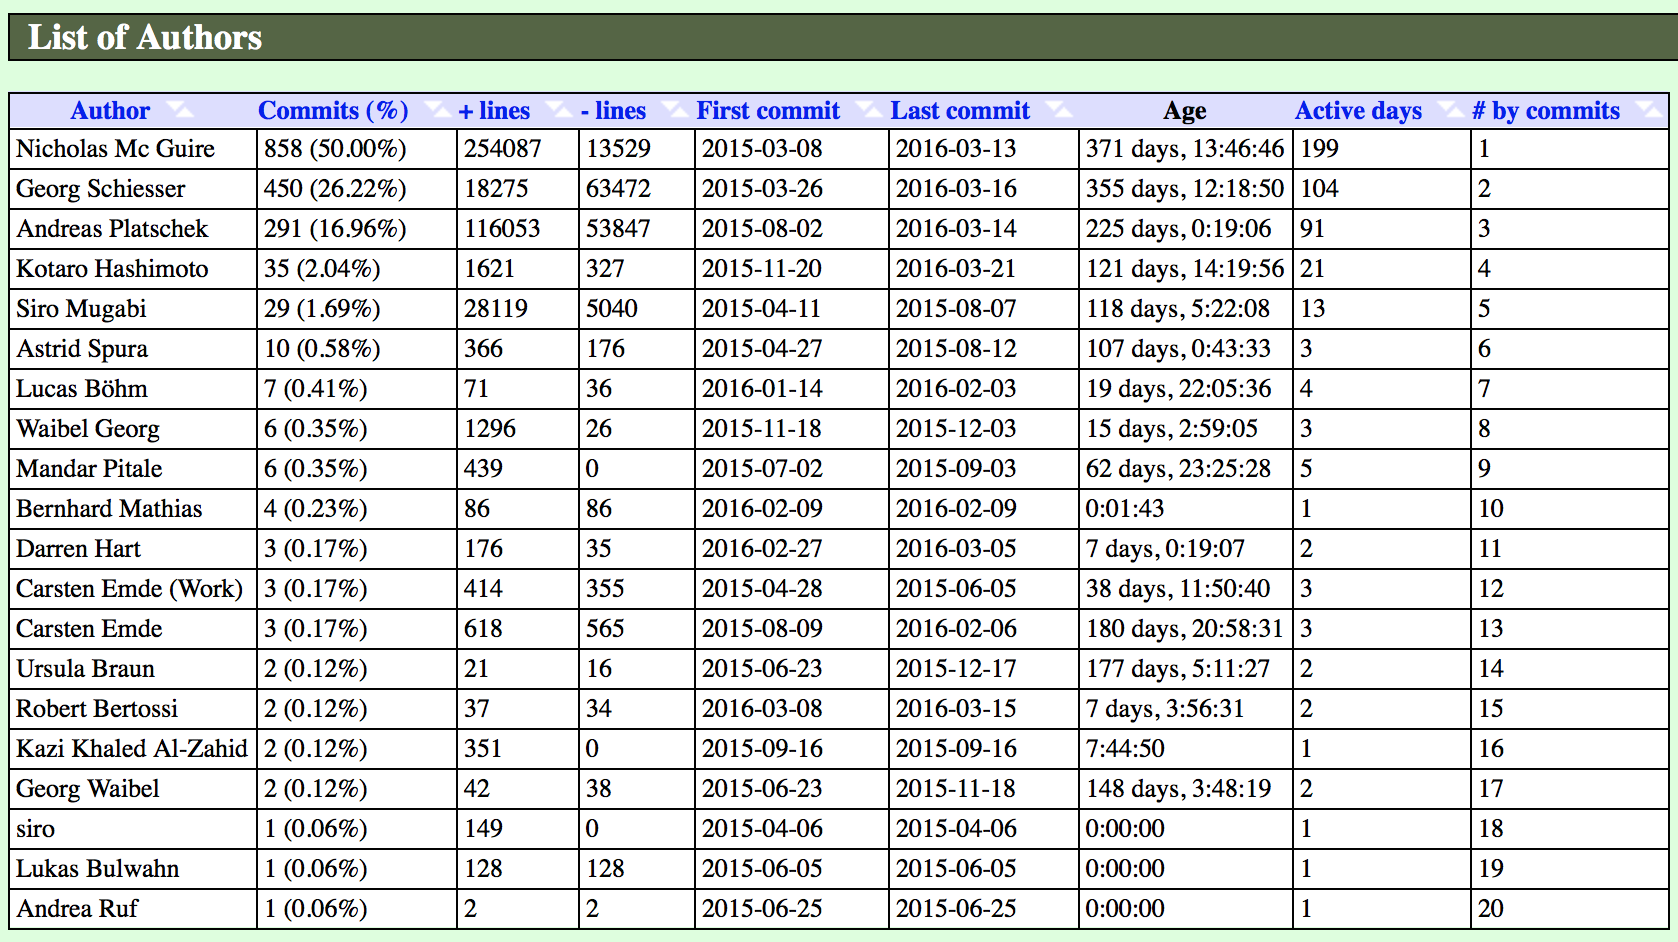
\includegraphics[width=\textwidth]{pic/gitstats.eps}
  \caption{開発者別\acrshort{sil2linuxmp} \acrshort{git}コミット寄与率集計結果}
  \label{gitstats}
\end{figure}
\par
コミット寄与率Top3のNicholas Mc Guire, Georg Schiesser, Andreas Platschekは\acrshort{sil2linuxmp}を主催する\acrshort{ot}のメンバーで、ドキュメント執筆、ツール調査・開発を主導している。
筆者(Kotaro Hashimoto)は35コミット(2.04\%)で、\acrshort{ot}メンバに続き4番目に寄与率が大きかった。
\ref{mailinglist}項でも述べたとおり、\acrshort{ot}と日立以外の参加企業からのコミットが非常に少ないことがプロジェクト上の懸念である。
今後\acrshort{sil2linuxmp}プロジェクトを盛り上げるために日立としてできる対策を考え、コミュニティが自発的に動き出すような仕掛けをしていくことがプロジェクト成功に不可欠である。
\subsection{Face to face meeting}
\acrshort{sil2linuxmp}プロジェクトは参加者間のコミュニケーションルートとしてメーリングリストと\acrshort{git}の他にface to face形式のミーティングやワークショップを重視している。
2016年3月第二週にはドイツ・ハイデルベルグでプロジェクト参加者全員を対象とするマイルストンミーティングが行われた。
ここでは\acrshort{sil2linuxmp}プロジェクトが始まってから約1年となるタイミングで、これまでの進捗と成果・残課題の共有および2年目の方針についての議論が行われた。
この場で日立からは\acrshort{codemini} Strategyと題した技術発表を行った。
\acrshort{codemini}技法は既存の様々なソフトウェア検証・解析手法のパフォーマンスを向上させる可能性を持ち、
機能安全認証プロセスにとっても非常に有効な戦略となり得る技術として\acrshort{sil2linuxmp}コミュニティから高い評価を受けた。
ミーティング終了後には\acrshort{ot}と日立とで別途会合を行い、より突っ込んだ質疑応答や意見交換を行った。
マイルストンミーティングでは、これまでメールと\acrshort{git}だけを介してコミュニケーションを取ってきた技術者と
直接顔を合わせて会話ができ、素朴な疑問や率直な意見をぶつけることでオンラインで行うよりも有意義な議論ができたと感じた。
